%!TEX program = xelatex
\documentclass[titlepage,11pt,a4paper]{article}
\usepackage{amssymb}
\usepackage{dsfont}
\usepackage{graphicx}
\usepackage[ruled,vlined]{algorithm2e}
\graphicspath{ {results/} }
\usepackage[titlepage]{polytechnique}


\title[INF 411 Programming Project]{Shortest Path Trees and Reach in Road Networks}
    %\subtitle{Le sous-titre (optionnel, enlever cette ligne sinon)}
    \author{Zuli \textsc{HUANG}\\
            Mingkun \textsc{LIU}
            }
    \date{09/01/2017}


\begin{document}
\maketitle

\section{Properties of Shortest-Path Trees}
To identify the number of different possible points we may be located in at the current moment of our trip, we choose the example vertex:
\begin{verbatim}
v 298251056 2277576 48783477
\end{verbatim}

\subsection{Question}{You have been traveling for time exactly t1 = 1 hour from the fixed starting point v towards your destination, which may be any sufficiently distant point in the network.}

We can obtain Figure \ref{fig:questioin_1.1_out} generated from the example vertex. Totally, there are 926 sufficiently distant points.
\begin{figure}[h]
    \centering
    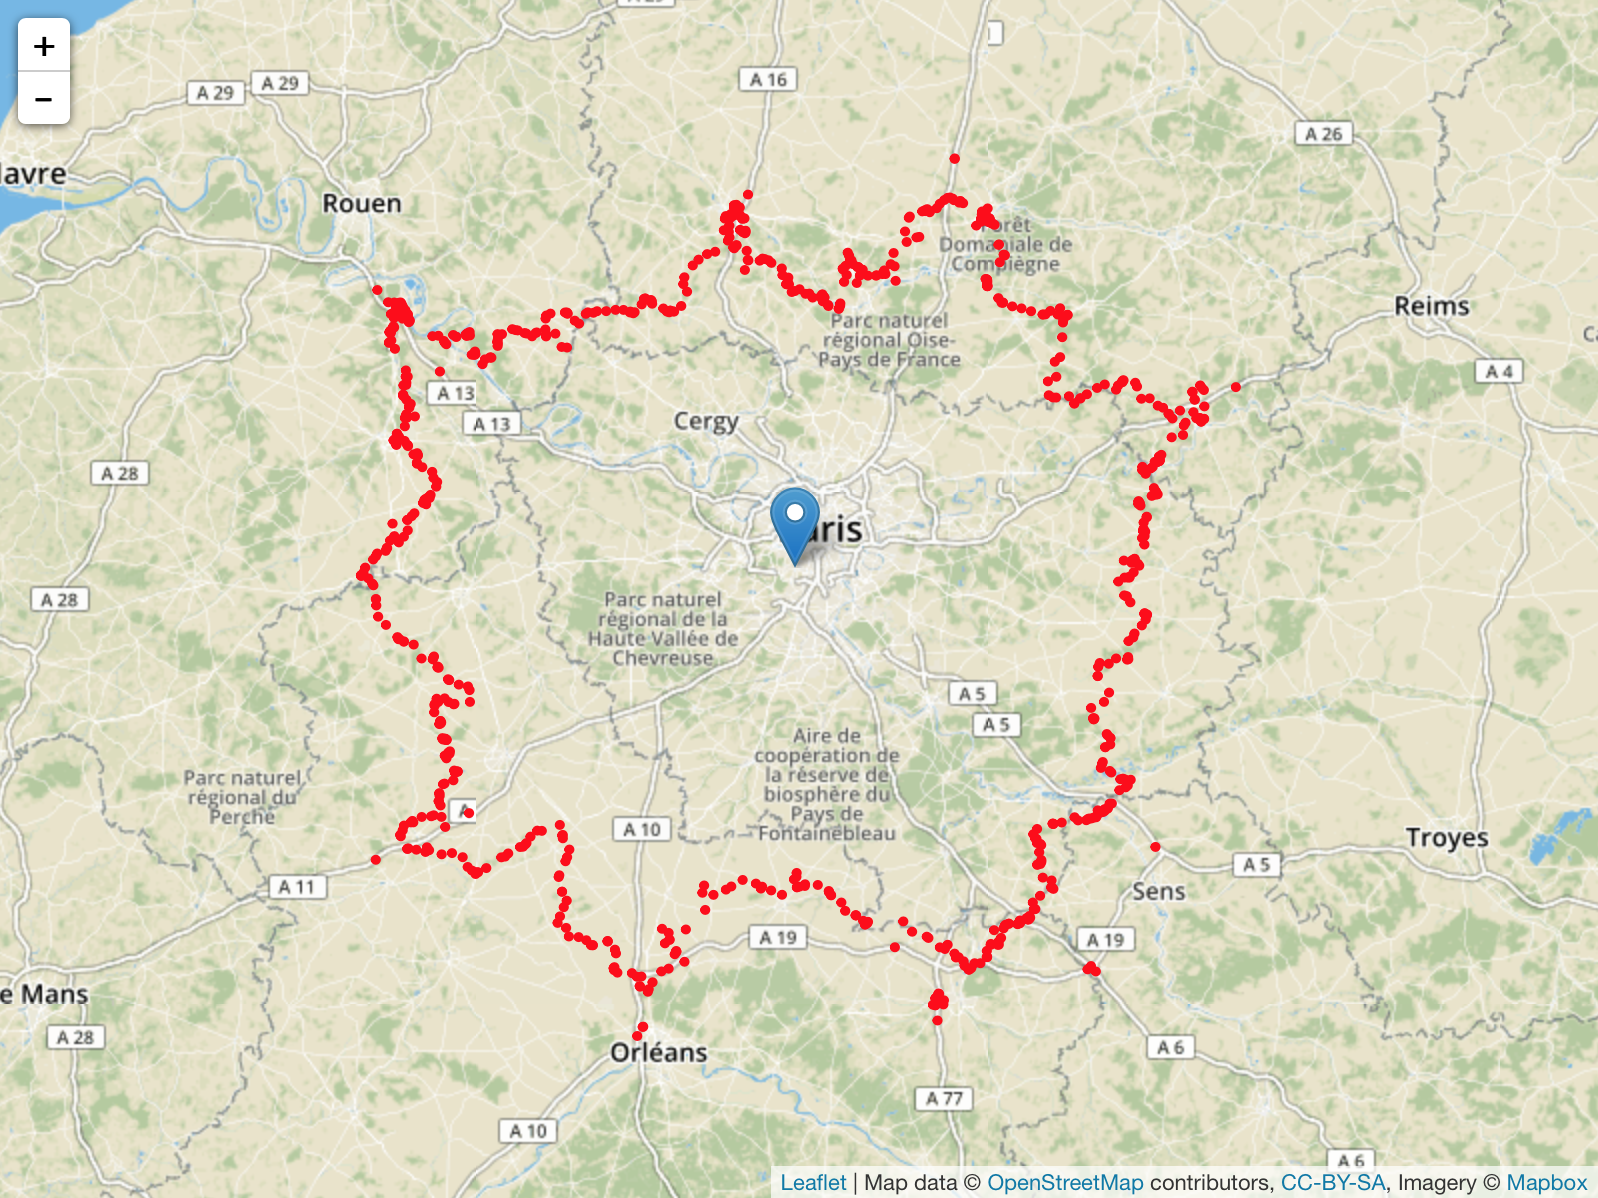
\includegraphics[width=\textwidth]{map_Q1.1.png}
    \caption{Points with 1h distance to vertex 298251056}
    \label{fig:questioin_1.1_out}
\end{figure}

\subsection{Question}{You have been traveling for time exactly t2 = 2 hours from the fixed starting point v towards your destination, which may be any sufficiently distant point in the network.}

It's similar to Q1.1. We choose the same center vertex v in the precedent question. And we obtain a map of sufficiently distant points. Totally, there are 2436 sufficiently distant ones.

\begin{figure}[h]
    \centering
    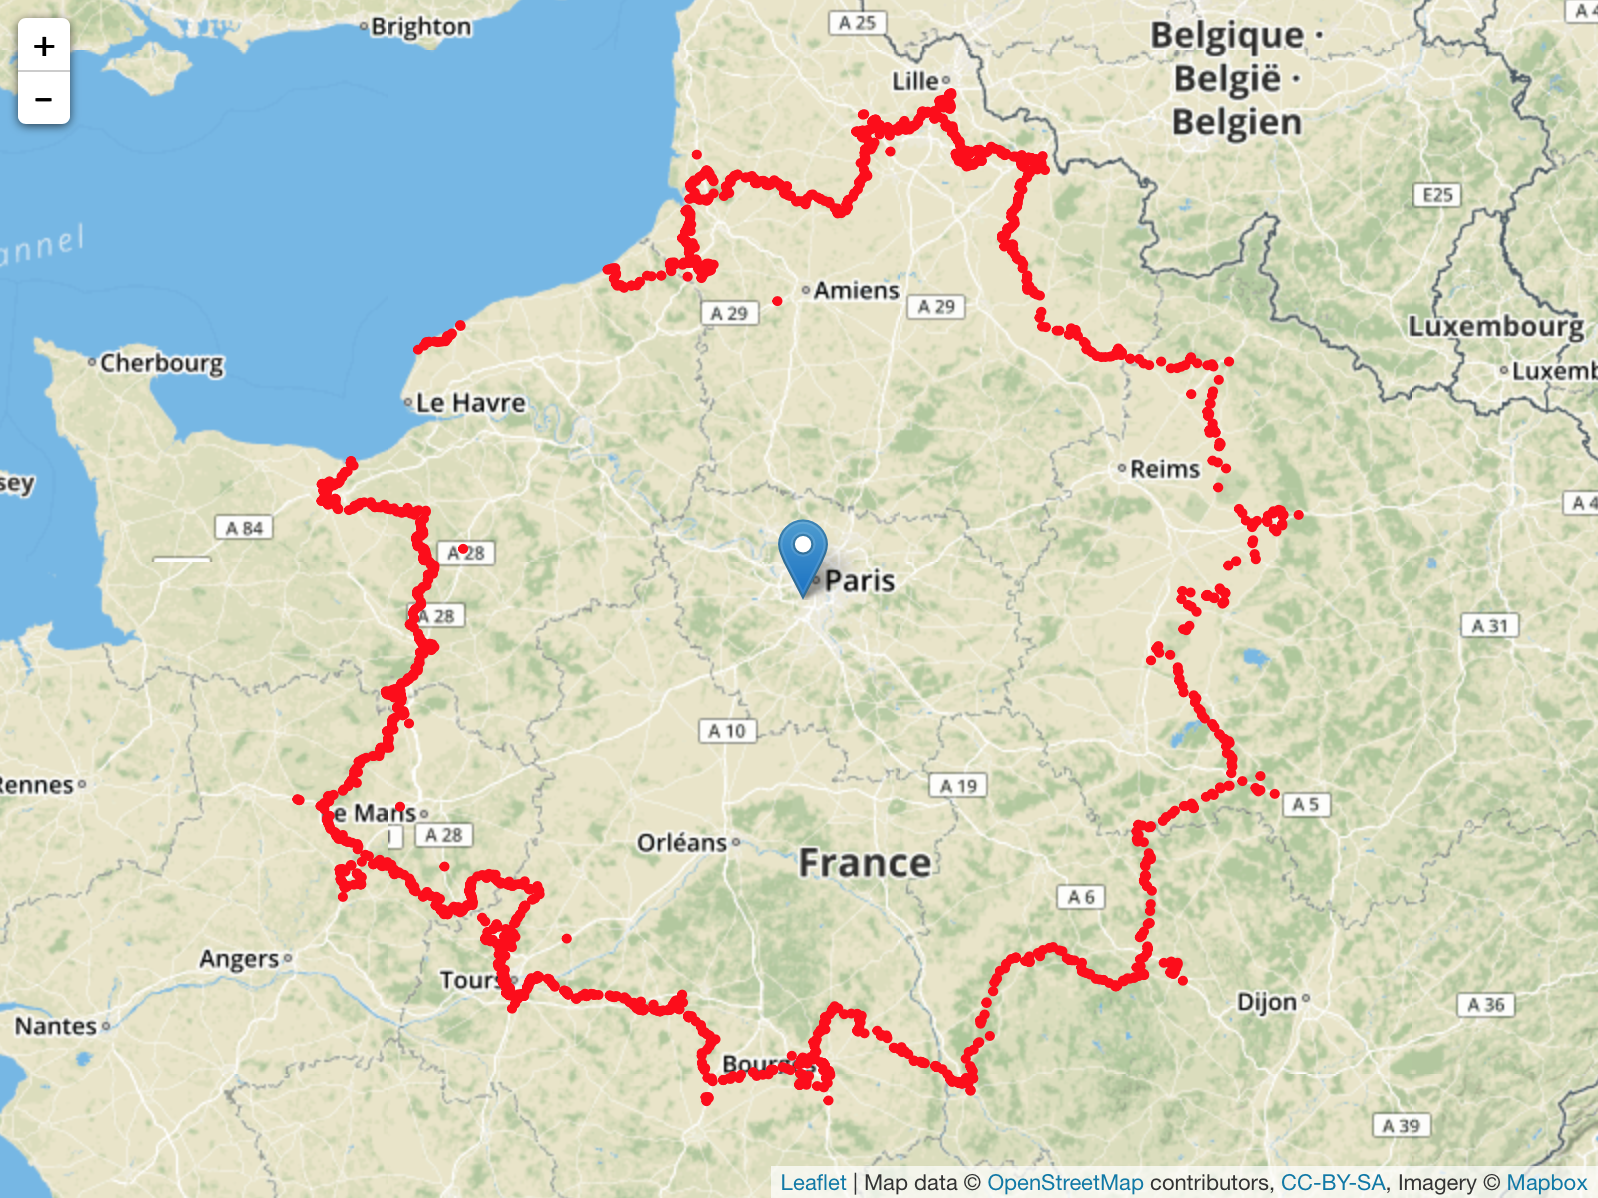
\includegraphics[width=\textwidth]{map_Q1.2.png}
    \caption{Points with 2h distance to vertex 298251056}
    \label{fig:questioin_1.2_out}
\end{figure}

\subsection{Question}{You have been traveling for time exactly t1 = 1 hour from the fixed starting point v towards your destination, when it is known that your destination is at least t2 = 2 hours' way away from your starting point v.}

We just need to back propagate points, obtained in the question 1.2, with 1h distance. And we get several appropriate points.

\newpage

\begin{figure}[h]
    \centering
    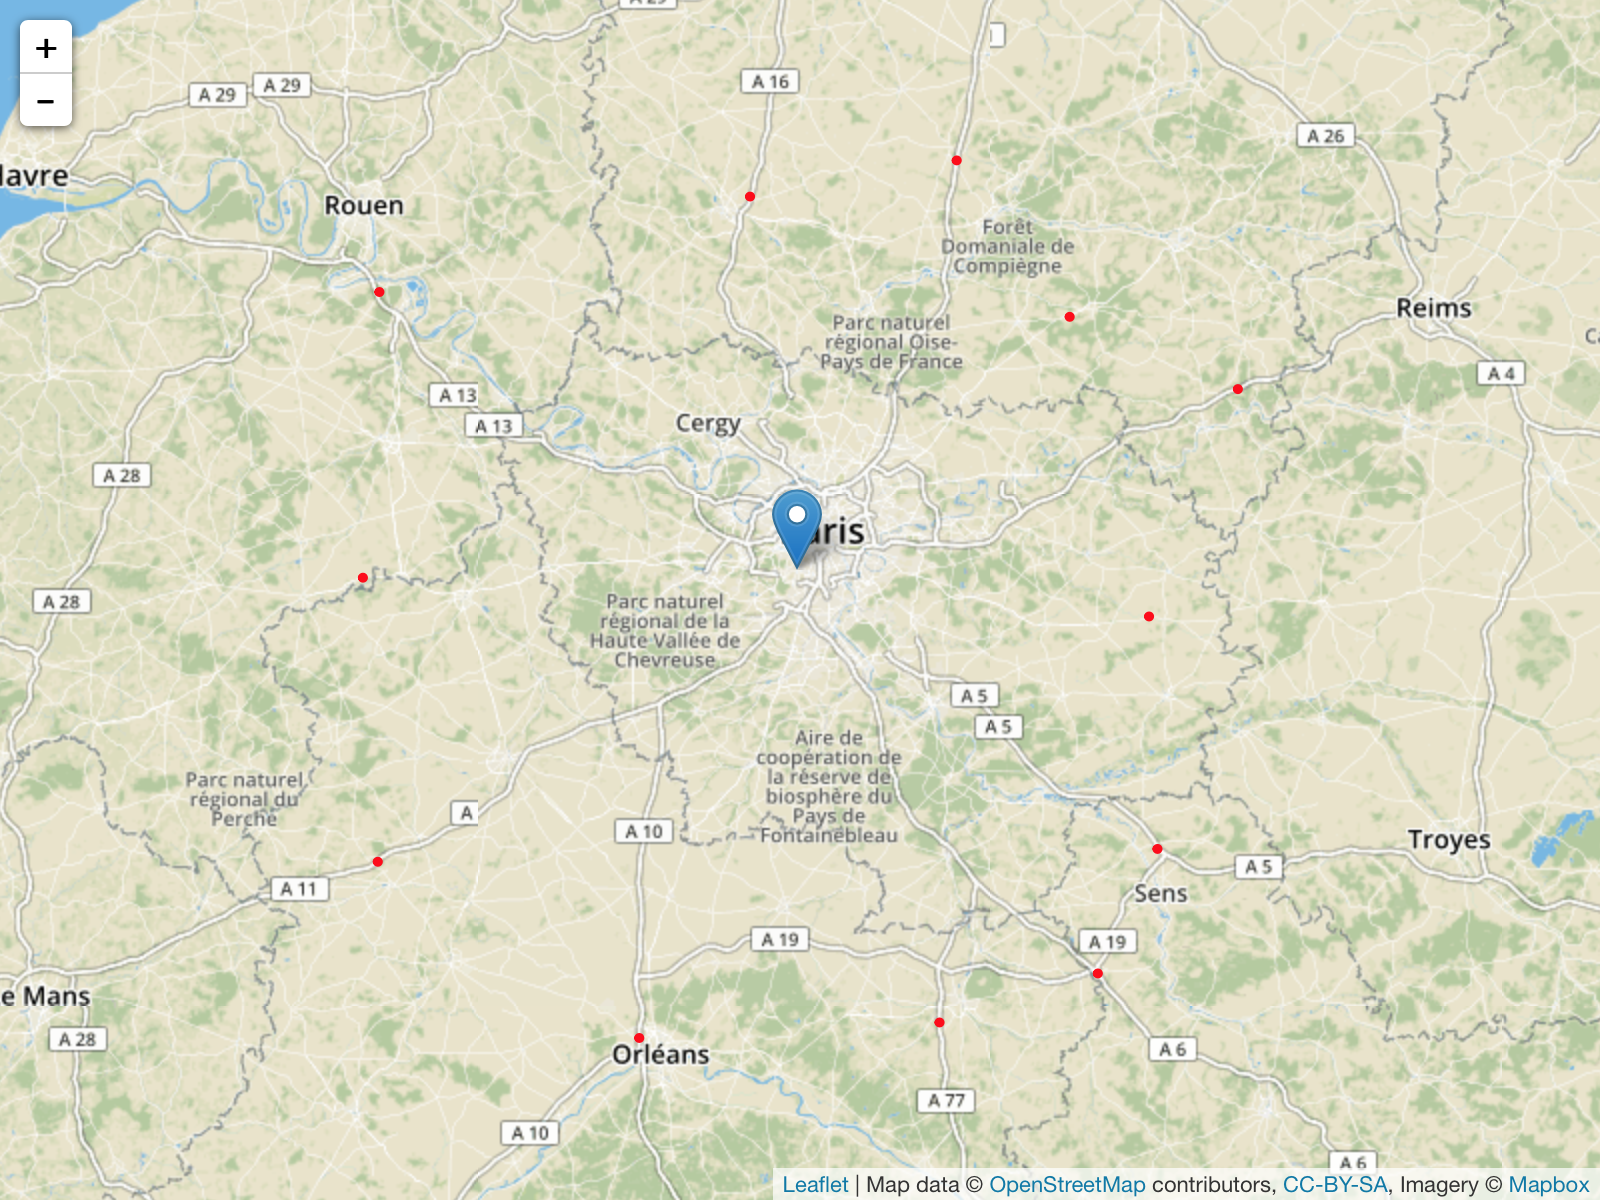
\includegraphics[width=\textwidth]{map_Q1.3.png}
    \caption{Points with 1h distance to v during a travel to a destination at least 2h away from v}
    \label{fig:questioin_1.3_out}
\end{figure}

\subsection{Methods}{Brief discussion of the graph algorithms used to answer the above questions.\\}
Algorithm that we use to handle question 1.1 to 1.3.

\begin{algorithm}[H]
 \KwData{An directed graph $G = (V, E)$, non negative wights, a source node $v\in V$, travel time $t$, $\omega : E \rightarrow \mathbb{R}$. Results generated in the algorithm: $d : V \rightarrow \mathbb{R}$ distance to v, $settled : V \rightarrow boolean$ and $p: V \rightarrow V$, predecessor of a vertex $x\in V$}
 \KwResult{Set of points with distance $t$ to $v$}

 \For{$x \in V$}{
  settled(x) := false\;
  d(x) := $\infty$\;
 }
 Q.initialize, Qb.initialize\;
 Q.add(v, v, 0)\;
 d(v) = 0\;
 \While{not Q.empty}{
  (x, prev, dist) := extractmin(Q, Qb)\;
  \eIf{$dist \leqslant d(x)$}{
    \If{$dist > t $ and $d(prev) \leqslant t$}{
      points.add(x, prev, t-d(prev)\;
    }
   }
   {
   continue\;
   }

  \eIf {settled(x)} {
    continue\;
  }
  {settled(x) := true}

  \For{$y \in N(x)$}{
    \If{not settled(y)}{

      \If{$\omega(x, y) + d(x) \leqslant d(y)$}{
      d[y]:=$\omega(x, y) + d(x)$

      \eIf {$d[x] \leqslant t$}{
          Q.add(y, x, $\omega(x, y) + d(x)$);
        }
        {
          Qb.add(y, x, $\omega(x, y) + d(x)$);
        }

      p[y]:=x

      }
    }
  }

 }
 return points\;
 \caption{Find points with a certain distance to a given vertex}
 \label{algo:vertices-distance}
\end{algorithm}

To find all sufficiently distant points without searching whole map, the main idea is to create two priority queues -- Q and Qb. Q stores the vertices whose predecessor that can be visited within the travel time limit. Qb stores the vertices whose predecessor that can't be visited within the travel time limit. It means that there is no more possible points when Q is empty. Another point is add a tuple element to priority queue, (vertex id, its predecessor id, distance). This point aims to successfully find those points, in different edge, that lead to the same vertex.


\begin{algorithm}[H]
 \KwData{An directed graph $G = (V, E)$, non negative wights, a source node v, a point $p$ with travel time t, $\omega : E \rightarrow \mathbb{R}$, $d : V \rightarrow \mathbb{R}$ distance to v and $p: V \rightarrow V$, predecessor of a vertex in $V$. The mother node of $p$ is vertex $x$ and the distance from $x$ to $p$ is $d_0$}
 \KwResult{A point with $p^*$ distance $t/2$ to $v$ in the path $v\rightarrow p$}

 dist := $t/2 - d_0$\;
 m := $p(x)$\;
 \While{$\omega(m, x) < $dist}{
  x := m\;
  m := $p(m)$\;
  dist := dist - $\omega(m, x)$\;
 }
 construct point $p^*$ from $(m, x, t/2 - d(m)$)\;
 return $p^*$\;
 \caption{Backward to a middle point}
 \label{algo:Backward}
\end{algorithm}

To solve question 1.3, first of all, we need to use Algorithm \ref{algo:vertices-distance} to get all points with 2h distance to source node v. Then, with function $p: V \rightarrow V$, we can get the predecessor of a settled vertex $x$ if $\mathrm{settle}(x) = true$. It means that we can finally find the middle point $p^*$ int the path $source\rightarrow p$ such that $\mathrm{distance}(p^*\rightarrow p) = 1h$ when $\mathrm{distance}(source \rightarrow p) = 2h$. We can use the following algorithm.





We can observe that there are few points obtained in Figure \ref{fig:questioin_1.3_out}. We can deduce that lots of vertices and edges will never be visited when we travel a sufficiently distant destination. And we find that the points in Figure \ref{fig:questioin_1.3_out} are all in "highways" connecting different cities.

\section{More theory and algorithms}

\subsection{B.1}
If the reach of a vertex is larger that $D/2$, by the definition of reach, there exists a fastest path through $v$ such that both of travel times from the starting point to $v$ and from $v$ to the destination are larger than $D/2$, which contradicts the assumption that $D$ is the diameter of the graph. This contradiction completes the proof.

\subsection{B.2}
If there exists a point $s$ in $S_{in}$ and a point $t$ in $S_{out}$ such that some quickest paths from $s$ to $t$ pass through $v$, then both of the travel times from $t$ to $v$ and from $v$ to $t$ are at least $1$ hour, which contradicts the assumption that the reach of $v$ is less than $1$ hour. This contradiction completes the proof.

\subsection{B.3}
Since the reach of $v$ is at least $2$ hours, there exists a fastest path through $v$ such that both of the travel times from the starting point to $v$ and from $v$ to the destination are at least $2$ hours. Since a subpath of a fastest path is also fastest, both of the paths from the starting point is $v$ and from $v$ to the destination are also fastest, and therefore, this path will pass through $S_{in}$ and $S_{out}$. This completes the proof.

\subsection{B.4}
Let $T_{out}(x)$ be the set of points to which the travel time from $v$ is exactly $x$ hours when traveling to a destination at least $2x$ hours' way away, and let $S_{in}(x)$ be the set of points from which the travel time to $v$ is precisely $v$ hour, when following a quickest path from a starting point located at least $2x$ hours' way from $v$.

By (B.2), if there exists a point $s$ in $S_{in}(x)$ and a point $t$ in $T_{out}(x)$, such that some quickest path from $s$ to $t$ passes through $v$, then the reach of $v$ is at least $x$ hours, if not, by (B.3), the reach of $v$ is less than $2x$ hours.

So for given $x$, we start with constructions of $S_{in}(x)$ and $T_{out}(x)$, and then find the shortest travel time from every point in $S_{in}(x)$ to every point in $T_{out}(x)$. If there exist $s\in S_{in}(x)$ and $t\in T_{out}(x)$ such that the travel time between $s$ and $t$ is $2x$, we have $r(v)\geq x$, and then we repeat the same steps but with $2x$ rather than $x$; if not, we have $r(v)\leq 2x$, and we repeat the same steps but with $x/2$ rather than $x$. Finally, we will reach a number $A$ that we have already calculated, and we return $2A$.


\begin{algorithm}[H]
 \KwData{a vertex $v$.}
 \KwResult{a value A such that $r(v)$ is in the range $[A/4, A)$.}
 Take $h=1$\;
 \While{true}{
  Construct $S_{in}(h)$ and $T_{out}(h)$\;
  Calculate the shortest travel time from every point in $S_{in}(h)$ to every point in $T_{out}(h)$\;
  \eIf{there exists a shortest travel time from a point in $S_{in}(h)$ to a point in $T_{out}(h)$ equals $2h$}{
   $h=2*h$\;
   }{
   $break$\;
  }
}


return $A := 2*h$\;

\caption{Find approximated value of reach}
\end{algorithm}

However, the approximation factor of this algorithm is $4$. If we would like to decrease this factor, we may repeat the loop with parameter $3A/4$, and if we repeat $\lceil\log(A/4)\rceil$ times, we will get the factor of $2$. Precisely, we can use the Algorithm \ref{algo:refine_algorithm} to repeat this precedure. As the distance and reach value can only be integer, we can finish the program within $\lceil\log(A/4)\rceil$ times.\\

\begin{algorithm}[H]
 \KwData{value $A$ such that $r(v)$ is in the range $[A/4, A)$.}
 \KwResult{value $A^*$ such that $r(v)$ is in the range $[A^*/2, A^*)$.}
 Take integer number $l=A/4, h=A/2$\;
 \While{$h>l$}{
 $\mathrm{mid}=\lfloor(l+h)/2\rfloor$\;
  Construct $S_{in}(\mathrm{mid})$ and $T_{out}(\mathrm{mid})$\;
  Calculate the shortest travel time from every point in $S_{in}(\mathrm{mid})$ to every point in $T_{out}(\mathrm{mid})$\;
  \eIf{there exists a shortest travel time from a point in $S_{in}(\mathrm{mid})$ to a point in $T_{out}(\mathrm{mid})$ equals $2*\mathrm{mid}$}{
   $l=\mathrm{mid}$\;
   }{
   $h=\mathrm{mid}$\;
  }
  return $2*\mathrm{mid}$;
}

return $A := 2*h$\;

\caption{Refine the approximation factor of reach}
\label{algo:refine_algorithm}
\end{algorithm}


\subsection{B.6}
Based on the results of (B.5), we have the following histogram:

\begin{figure}[h]
    \centering
    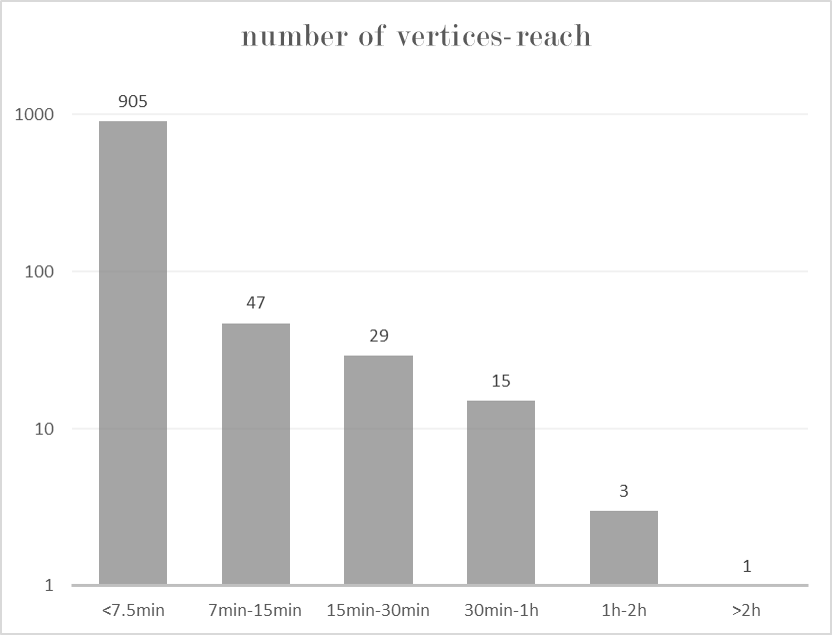
\includegraphics[width =0.75\textwidth]{reach.png}
    \caption{histogram of number of vertices-reach}
    \label{fig:reach}
\end{figure}

\end{document}
